
\documentclass[10pt,twoside,twocolumn]{article}
\usepackage[left=.75in,top=.75in,right=.75in,bottom=.75in]{geometry} % Document margins
\usepackage{hyperref}
\usepackage{url}
\usepackage{float}
\usepackage{tikz}
\usetikzlibrary{fit,positioning,shapes}
\usetikzlibrary{arrows,automata}
\usepackage{amsmath}
\usepackage{ dsfont }
\geometry{a4paper} % or letter or a5paper or ... etc

\title{Alexa Socialbot}
\author{Carter Brown \and Abhimanyu Gupta \and Sumner Hearth \and Charles Howland \and Ishaan Jhaveri \and George Li \and Julian Moraes}
\date{%
    Cornell University\\%
    \today
}% delete this line to display the current date

\begin{document}
\maketitle

\section{Overview}
The overall design of the conversational module is to break different aspects of the conversational requirements into one of two sections: CC (chit-chat) or DD (data-driven). These reflect our view of the two principal components of a conversation: phrasing responses and incorporating relevant data. The CC module is responsible for creating cohesive sentences in response to the user. The DD section is responsible for finding relevant data and facts as required for formulating a response.

\section{CC Overview}
This module, called "Chit Chat" (CC) serves to generate context-sensitive responses to user queries to engage users and drive continued discourse. The model builds off basic seq2seq models such as \cite{Vinyals2015} to more sophisticated architectures such as the DCGM \cite{Sordoni2015}, TACNTN \cite{Wu}, vector embeddings of users' personas and sentiments \cite{Li2016a}, and experimenting with reinforcement learning in the network training \cite{Zaremba2015, Williams2016, Li2016b}. There is a local DMN \cite{Kumar:2015, Xiong2016} to keep track of recent information in the conversation that can be called quickly. Furthermore, this component will provide a vector embedding framework for phrasing responses when we must query the DD module and inject information into the conversation.

\section{CC Architecture}

Text first runs through a classifier to determine whether a proper response to the query requires information "outside" the conversation, i.e. real-world info not recently mentioned in the conversation. This can be accomplished by a mix of classical NLP classifiers coupled with a search through the local user DMN present in this module for a relevant answer. If more information is required, then it is passed onto the DD module.

\noindent
In both cases, the flow of information returns to the CC module to be merged together. If classic information retrieval among tuples a la Freebase API is effective, then we will return that answer as has been solved in \cite{Iyyer2014, Yao2014a, Yao2014b}. On the other hand, accessing a response from our DD memory bank in figure~\ref{DD_design}, requires more innovative integration of information.

\noindent
This is where our vector embedding comes into play!

\begin{figure}[H]
    \centering
    \resizebox{180pt}{110pt}{
    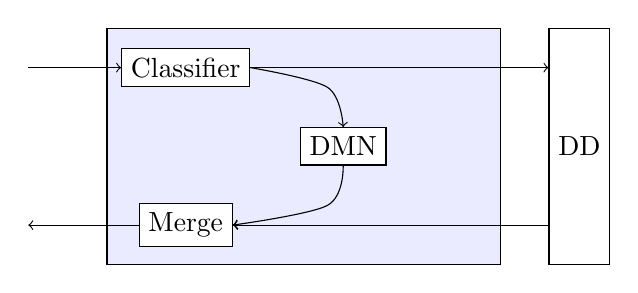
\begin{tikzpicture}
        \tikzstyle{every node} = [draw,shape=rectangle,fill=white]
    \filldraw[fill=blue!40!white, draw=black, opacity=0.2] (1,0) rectangle (6,3);
    \draw (1,0) rectangle (6,3);
    
    \node (CCDD) at (2,2.5) {Classifier};
    \node (DMN) at (4,1.5) {DMN};
    \node (toDD) at (7,2.5) {DD};
    \node (fromDD) at (7,0.5) {DD};
    \node[minimum height=3cm] (DDcheat) at (7,1.5) {DD};
    \node (merge) at (2,0.5) {Merge};

    \draw [->] (0,2.5) -- (CCDD);
    \draw [->] (CCDD) -- (toDD);
    \draw [->] (fromDD) -- (merge);
    \draw [->] (merge) -- (0,0.5);
    \draw [->] plot [smooth,tension=.55] coordinates {(CCDD.east) (3.8,2.25) (DMN.north)};
    \draw [->] plot [smooth,tension=.55] coordinates {(DMN.south) (3.8,0.75) (merge.east)};

    \end{tikzpicture}
    }
    
    \label{CCdesign}
    \caption{CC architecture}
\end{figure}

\section{DD Overview}
The Data Driven module (DD) incorporates outside data and information into the conversation. The module assumes that the user's query has been classified in the CC module to require additional information that the standard conversational net cannot provide. DD makes use of recent advances in Neural Network memory systems and topic classification.

\noindent
A bank of Dynamic Memory Networks (DMNs) \cite{Kumar:2015, Xiong2016} store information on various topics that the user can query. A Topic Classifier (TC) chooses which DMN to use, and will be implemented using SVMs\cite{Joachims1998, Pilaszy2005}, LDA\cite{Blei2001, Zhao2011}, or possibly CNNs\cite{Kim2014}. Note that the architecture is ``black-boxed'' and specific implementation details will be determined through iterative testing (see Methodology).

\section{DD Architecture}
The architecture of the Data Driven (DD) section of the conversational system is given by figure~2. The topic nodes represent Dynamic Memory Networks (DMNs) \cite{Kumar:2015, Xiong2016}, and the TC node is a topic classifier to dispatch commands to one of the provided topics.

\noindent
After the preprocessing of the previous module, English text from the user's query is passed into the Topic Classifier (TC). The TC determines the topic, i.e. some class, of the user's query. The classes are predefined from training and this section is black-boxed for the sake of this general architecture. However, it seems that \cite{Zhao2011} provides an interesting and potentially fruitful framework for classification on short text segments. Furthermore, for each of these classes from training is a DMN+ \cite{Xiong2016} containing relevant information that we also obtained from training. This training can again be black-boxed for the sake of this design, but different avenues we will investigate include querying Google, Wikipedia, or something else we come up with during training as we see which websites and precreated databases contain the best information.

\noindent
Furthermore, there are DMN+'s on current event topics, such as pop culture, politics, etc. The DMN+'s are continuously updated with information. This captures the idea that important information persists through the DMN+ from day-to-day. Since there has been no research on how large the DMN+'s can effectively be, we will have to determine this once we get to actually training and implementing. To accommodate this issue, we propose making our topic classifier more fine-grained if possible. If this is not reasonable, then augmenting DMN+'s with more traditional, ``non-neural'' QA architectures, such as those found in \cite{Iyyer2014, Yao2014a, Yao2014b}. However, all of these would require a slight implementation change on a technical scale since these architectures require Freebase API, which we had downloaded before Google removed access to it, and has a different underlying representation of the data.

\noindent
Some work such as \cite{Zhang2016} has brought together a knowledge base with a neural net to produce QA responses before. However, our approach differs in encapsulating the attention mechanism within the DMN+ bank. Furthermore, while \cite{Zhang2016} proposes a method to solve the Out of Vocabulary (OOV) problem, it does not appear to accommodate this problem on queries from the user. To remedy this, we propose overlaying the DMN+ \cite{Xiong2016} with a Pointer Sentinel Mixture Model \cite{Merity2016}. Since the Pointer Sentinel Mixture Model (PSMM) can augment any architecture with a softmax layer, this with the answer module of our softmax, the output of which feeds back into a GRU. Since the PSMM has been merged only with LSTM's before, this new architecture feature should make our DMN+ information retrieval bank more robust.



\subsection{Topic and DMN Distribution}
The Topic DMN+'s can be separated into two groups: Global modules and User modules. In figure~2, the left side and right side are two different levels of distrubtion--local, and global, respectively.

\noindent
Global modules are populated with information deemed relevant to all users' interests, such as sports, politics, and culture. These modules can be queried by any DD module for any user and the same responses should be expected (i.e. ``Who won the game on Saturday'' is not user-dependent). As such these modules can be shared among all instances of the DD module.

\noindent
User modules are tailored to a specific user's interests, stored locally for the user. The TC module can double as a simple unsupervised learning system as well as a labeled topic classifier in order to determine what topics a specific user may find interesting. Hence, these classifications evolve with the user as they interact more with Alexa. These topics can then be researched and added to the list of available topic DMNs.

\begin{figure}
    \centering
    \resizebox{160pt}{135pt}{
    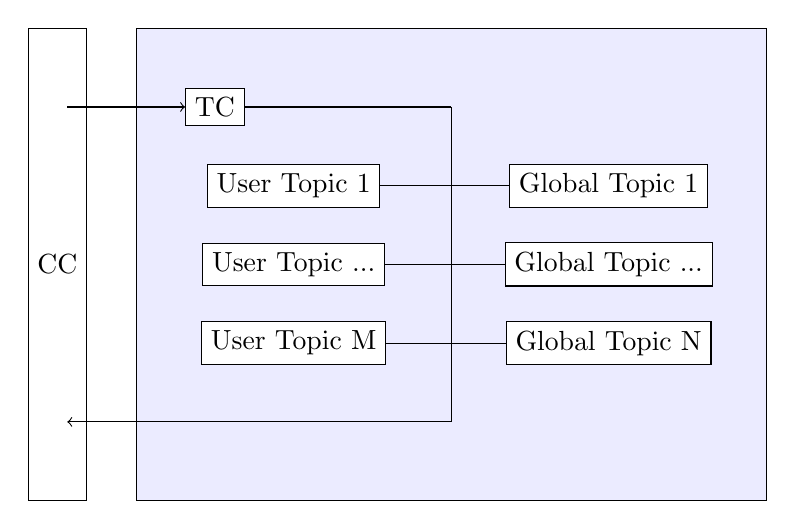
\begin{tikzpicture}
    	\tikzstyle{every node} = [draw,shape=rectangle,fill=white]
	\filldraw[fill=blue!40!white, draw=black, opacity=0.2] (1,0) rectangle (9,6);
	\draw (1,0) rectangle (9,6);
	
	\node (TC) at (2,5) {TC};
    
    \node (CC1) at (0,5) {};
    \node (CC2) at (0,1) {};
    \node[minimum height=6cm] (CC) at (0,3) {CC};
	
	\node (Topic1) at (7,4) {Global  Topic 1};
	\node (TopicE) at (7,3) {Global Topic ...};
	\node (TopicN) at (7,2) {Global Topic N};
	
	\node (UTopic1) at (3,4) {User Topic 1};
	\node (UTopicE) at (3,3) {User Topic ...};
	\node (UTopic2) at (3,2) {User Topic M};
	
	\draw [->] (CC1) -- (TC);
	\draw (TC) -- (5,5); 
    \draw (5,5) -- (5,1);
	\draw [->] (5,1) -- (CC2);
	\draw (Topic1) -- (5,4);
	\draw (TopicE) -- (5,3);
	\draw (TopicN) -- (5,2);
	\draw (UTopic1) -- (5,4);
	\draw (UTopicE) -- (5,3);
	\draw (UTopic2) -- (5,2);
	
    \end{tikzpicture}
    }
    
    \label{DDdesign}
    \caption{DD architecture}
\end{figure}

\section{Information Gathering \label{section_info}}
Populating the DMNs is a constant process. The general implementation will be to discover facts on a topic via predefined news sources (i.e. Google News) or databases (i.e. Wikipedia) and to convert any fact tables into simple sentences. This means that information such as the tuple \emph{(Country: United States, Capital: Washington D.C.)} should be entered into the DMN as \emph{``The capital of the United States is Washington D.C.''}. Global topics should be constantly querying for the most relevant information, weighted by importance and age. More important topics should remain in the DMN longer, and more recent topics should be included. Should a query not find results in the topic's DMN then more classical Information Retrieval algorithms can be employed to compute the result and populate a user DMN for later reference. User DMNs will have a twofold responsibility. They will cover topics not relevant to the general population or which are more specific than generally necessary.
These user topics can be populated during a conversation, but also when the user is not active. Using the preexisting TC module we can query incoming news or database entries for information deemed relevant and important and populate the appropriate DMN for later conversations. 

\bibliographystyle{plain}
\bibliography{bib} 

\end{document}